\documentclass{article}
\usepackage{amsfonts}
\usepackage{amsmath}
\usepackage{xcolor}

\usepackage{enumitem}

\usepackage{graphicx}
\graphicspath{{./images/}}
\usepackage{sidecap}

\usepackage{hyperref}

\usepackage{listings}
% \lstset{
%   % basicstyle=\ttfamily,
%   % columns=fullflexible,
%   % frame=single,
%   breaklines=true,
%   postbreak=\mbox{\textcolor{red}{$\hookrightarrow$}\space}
% }
\lstset{
  basicstyle=\ttfamily,
  breaklines=true,
  postbreak=\mbox{\textcolor{red}{$\hookrightarrow$}\space},
  stepnumber=1,
  tabsize=1,
}

\usepackage[margin=1in]{geometry}

\usepackage{float}

\title{Real-Time Procedural Terrain Generation with Marching Cubes}
\author{Joseph Chambers-Graham}
\date{}

\setcounter{tocdepth}{3}

\begin{document}

\bibliographystyle{plainurl}

\maketitle
\newpage

\section*{Abstract}
This project explores a method for procedurally generating terrain by applying the a variation of the Marching Cubes algorithm known as the Transvoxel algorithm. We use an octree data structure to break down a large world into chunks at varying levels of detail, and apply the parallel processing power of the GPU to rapidly generate geometry on a per-chunk basis. We then explore applications of this approach, modifying the geometry in real-time by making localized changes to the underlying distance function. %Finally, we demonstrate the applicability of this approach by 
Finally, we use the meshes we have generated with a well-known physics library.
\newpage

\tableofcontents

\newpage
\section{Introduction}
- project and report overview
\section{Background}
\subsection{Signed Distance Functions}
\label{section:sdf}
At the core of the Marching Cubes algorithm, and the way we will be defining shapes, is the signed distance function (SDF). This is a function of the form $f:\mathbb{R}^3 \rightarrow \mathbb{R}$. The shape represented by an SDF is the implicit surface $f\left(x,y,z\right) = 0$. Furthermore, it is desirable for an SDF to have the following properties:
\begin{enumerate}[label=\roman*.]
\item At all points where $f\left(x,y,z\right) \neq 0$, if $\left(x,y,z\right)$ is inside the surface, $f\left(x,y,z\right) < 0$. If $\left(x,y,z\right)$ is outside the surface, $f\left(x,y,z\right) > 0$. This is the most important property of an SDF, without which the Marching Cubes algorithm is unlikely to produce valid geometry.
\item At all points where $f\left(x,y,z\right) \neq 0$, the value $f\left(x,y,z\right)$ should be the smallest (signed) euclidean distance from the point $\left(x,y,z\right)$ to the surface $f\left(x,y,z\right) = 0$. In practice, many implicit functions we are using do not have this property, however for best results the value $f\left(x,y,z\right)$ should be a good approximation of the actual distance, and for floating point precision reasons, must be at least the same order of magnitude. This property will be used by the Marching Cubes algorithm to interpolate the positions of vertices, and as such a better distance approximation will lead to a more accurate mesh representation of the SDF. An SDF such that $f\left(x,y,z\right)$ gives the correct distance everywhere is an \textit{exact} SDF. Otherwise, it is an \textit{approximate} SDF.
\item $f$ is continuous everywhere, and has all partial derivatives. This is useful for calculating the normal to the surface at a given point. In practice, we will relax these restrictions, but this should still hold in places where the algorithm might generate vertices.
\end{enumerate}
Many primitive shapes have exact SDF representations \cite{quilez:sdf}. Figure \ref{fig:Circle_SDF} shows a 2 dimensional exact SDF for a circle.

\begin{SCfigure}[][H]
\caption{Example of a 2 dimensional SDF representing a circle. The function shown is $f\left(x,y\right) = \sqrt{x^2+y^2}-1$, with the area where $f\left(x,y\right) < 0 $ shaded. Also shown are the contours where $f\left(x,y\right) = 0.1,0.2,...0.5$}
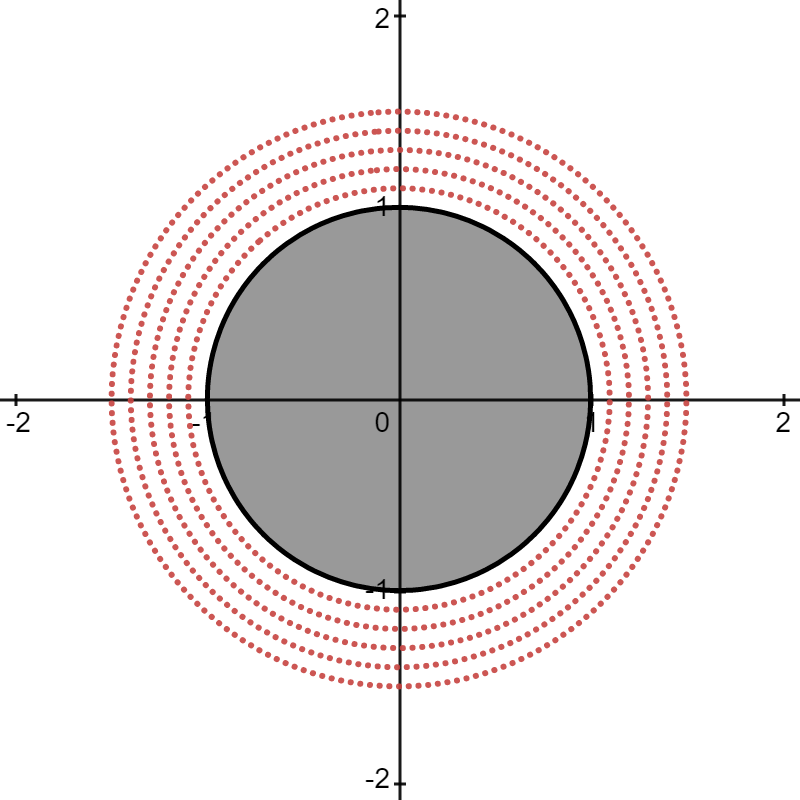
\includegraphics[width=0.5\textwidth]{Circle_SDF}
\label{fig:Circle_SDF}
\end{SCfigure}

However, many useful shapes, in particular heightmaps and shapes those defined by random noise, are not easy to represent as an exact SDF. For this sort of shape, we use an approximate SDF. Figure \ref{fig:Hill_SDF} shows a 2 dimensional approximate SDF for the heightmap defined by $y=1-\frac{x^2}{3}$. It is of course possible to define the exact distance function for any implicit shape, however such problems are often minimisation problems with with solutions that are expensive to compute. For example,even this simple example computing the exact distance to a quadratic curve requires computing the roots of a cubic polynomial, and computing the exact distance to a cubic curve requires solving a polynomial of degree 5, for which there is no elementary solution. Since this is useful for defining shapes based on interpolation splines, it is certainly worth considering when an approximation may be worth using due to the reduced computational cost.

\begin{SCfigure}[][H]
\caption{Plot of the SDF $f\left(x,y\right) = y - \left(1 - \frac{x^2}{3}\right)$. Note the contour lines are no longer uniformly spaced, as they would be with an exact SDF. In fact, the distance approximation gets worse, as the slope of the surface increases.}
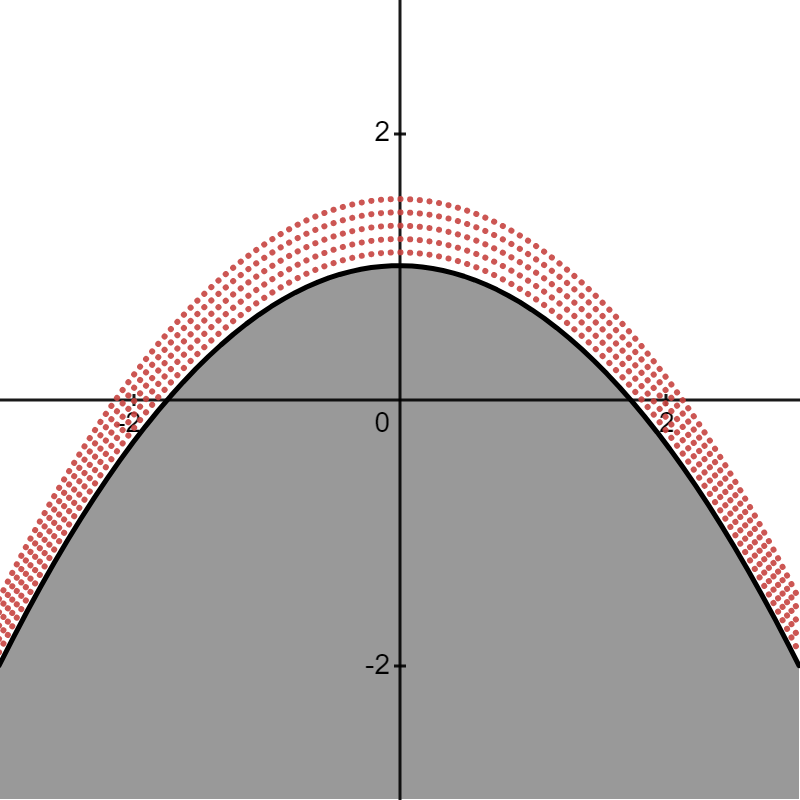
\includegraphics[width=0.5\textwidth]{Hill_SDF}
\label{fig:Hill_SDF}
\end{SCfigure}

The basic set-theoretical operations of union, intersection, and difference have equivalent representations using the $\min$ and $\max$ functions. At this point, one many note that the function $\min\left(f,g\right)$ may fail to be differentiable at the point where $f = g$. Here, we may simply take the derivative of $f$ or $g$. 
\\
It is worth noting that some literature chooses the terminology of signed \textit{density} functions \cite{nguyen_geiss_2007}. This is equivalent to an approximate SDF, however the sign convention is flipped, so that a negative value is outside the surface.\\
%https://developer.nvidia.com/gpugems/gpugems3/part-i-geometry/chapter-1-generating-complex-procedural-terrains-using-gpu

\subsection{Noise}
A typical noise function takes as input a point in $\mathbb{R}^n$ and returns a pseudorandom value, usually between 0 and 1. The use of noise to generate convincing heightmaps is well-documented, and typical implementations are as a function of the form $y = h\left(x,z\right)$ giving the height of the terrain at a given $\left(x,z\right)$ coordinate. This can be simply extended to an approximate SDF, using the formula $f\left(x,y,z\right) = y - h\left(x,z\right)$. Note that this is in fact an approximate SDF, and that the distance approximation worsens as the steepness of the slope of $h\left(x,z\right)$ increases. This phenomenon can be seen in figure \ref{fig:Hill_SDF}.
\\
The use of 3 dimensional noise as a distance function is also possible, and yields interesting results. %TODO - implement  this

\subsection{Marching Cubes Algorithm}
\label{section:mc}
The Marching Cubes algorithm is an algorithm for polygonising a 3 dimensional scalar field. It works by splitting the space into a uniform grid of cubes (\textit{cells}), and sampling the scalar field at the vertices of each cube. Pre-computed lookup tables, indexed by the vertices of the cell which are classified as "inside" or "outside", are used to determine the geometry that exists within the cell. Each vertex of this geometry lies on an edge of the cell, and the position of each geometry vertex is adjusted by linearly interpolating the sampled values of the scalar field at the cell vertices, such that the vertex is placed approximately on the surface described by the scalar field. In this project, we use a 3 dimensional SDF as described in Section \ref{section:sdf} to provide scalar field samples, and the lookup tables as described by Paul Bourke. \cite{bourke_1994}

\section{Design}
\subsection{GPU Implementation}
\label{section:mc_gpu}
The Marching Cubes algorithm operates on a large grid of cells, on a per-cell basis. As such, it is well-suited to parallelisation. In this section, we describe an implementation of the Marching Cubes algorithm on a GPU, using GLSL. This implementation is based on the reference implementation cited in Section \ref{section:mc}. The implementation works on \textit{chunks}, which are cuboids of grid cells, and is split into 3 phases:
\begin{enumerate}

\item \underline{Distance function computation}: For each grid cell vertex in the chunk, the SDF is sampled, and the values are stored in a buffer to be passed to the subsequent phases. This is done separately to the other phases, which operate over grid cells rather than grid cell vertices, to avoid unnecessary recomputation of the SDF, since one grid cell vertex may belong to up to 8 neighboring grid cells.
\begin{lstlisting}[language=C++,label={mc_generate},caption={GLSL code for generating the SDF at one vertex in a chunk. The function \texttt{generate} may use any SDF, and stores the value in a buffer.}]
void main() {
  uvec3 gid = gl_GlobalInvocationID;
  if (gid.x > chunkSize.x || gid.y > chunkSize.y || gid.z > chunkSize.z) {
    return;
  }
  generate(gid);
}
\end{lstlisting}

\item \underline{Counting phase}: For each grid cell in the chunk, the number of mesh triangles in the cell is calculated, using the SDF sample values computed in the previous phase. This allows the vertex buffer to be sized correctly. This phase also filters out grid cells which have no triangles in at all, since no geometry needs to be generated. Listing \ref{mc_count} shows part of the code responsible for this. Variable \texttt{cubeIndex} is calculated according to the Marching Cubes algorithm, and corresponds to the vertices of the grid cell that are inside or outside of the surface. Hence, this \textit{cube index} determines the geometry that will end up in each grid cell. \texttt{totalTable} contains the number of triangles in a grid cell with that index, which is added to the atomic variable \texttt{pointCount}. \texttt{bufferIndex} reserves a place in the buffer \texttt{marchableList} for this grid cell. The condition in line 1 filters out the cube indices which do not generate any geometry.
\begin{lstlisting}[language=C++,label={mc_count},caption={GLSL code for counting the number of vertices and marchable grid cells in the chunk.}]
if (cubeIndex != 0 && cubeIndex != 255)
{
  atomicCounterAddARB(pointCount,totalTable[cubeIndex]);
  uint bufferIndex = atomicCounterIncrement(marchableCount);
  uvec4 mc = uvec4(gid.x,gid.y,gid.z,cubeIndex);
  marchableList[bufferIndex] = mc;
}
\end{lstlisting}

\item \underline{Polygonisation phase}: For each of the grid cells that will contain mesh triangles, these triangles are actually generated, and the vertex positions are adjusted by linearly interpolating the pre-computed SDF values. At this stage, the vertex normals are also generated. This can be done using face normals, or by providing a normal function. Listing \ref{mc_poly} shows part of the code responsible for this. Atomic variable \texttt{triCount} keeps track of the number of triangles that have been generated across the entire chunk, and allocates a space in the buffers \texttt{vertices} and \texttt{normals}, which have been sized according to the values calculated in the previous phase. \texttt{triTable} is a buffer containing a flattened version of the table with the same name in the reference implementation. It contains a list of indices into the array \texttt{vertlist} for each cube index. Each vertex in \texttt{vertlist} is positioned on the edge of the grid cell, linearly interpolated as described in Section \ref{section:mc}.
\begin{lstlisting}[language=C++,label={mc_poly},caption={GLSL code for generating the geometry of a grid cell.}]
for (int tCount = 0; triTable[tCount+16*cubeIndex] != -1; tCount+=3)
{
  uint index = atomicCounterIncrement(triCount);
  for (int t = 0; t < 3;t++)
  {
    vec3 vertPos = vertlist[triTable[cubeIndex*16+tCount+t]]*chunkStride + chunkPosition;
    vertices[3*index+t] = vec4(vertPos,1);
    normals[3*index+t] = vec4(modified_normal(vertPos),0);
  }
}
\end{lstlisting}

\end{enumerate}
The choice to parallelise the algorithm in this way presents some downsides. Triangles are generated and placed into the vertex buffer in an order which is very unlikely to be coherent, meaning that there is no way to reliably use an index buffer for vertices that are generated in the same place, a common occurance. This results in many duplicate vertices in the vertex array. Nevertheless, this is a worthwhile tradeoff, with the GPU implementation greatly outperforming the CPU implementation. 
\subsubsection{Comparison of CPU and GPU implementations}
The SDF used for these comparison tests is a scaled 3D noise function. Pseudorandom numbers for this noise function are generated using combinations of built in floating point functions in GLSL in the GPU implementation, and functions from the GLM C++ library in the CPU implementation. An effort has been made to ensure these functions are equivalent, however due to floating point inaccuracies and differences between these implementations, the SDF occasionally produces slightly different values between implementations, and this results in the number of triangles generated being slightly different also. However, this difference is very small compared to the total number of triangles generated, so is unlikely to have a significant impact on the runtime comparison. For example, the largest test, generating 1000 chunks of size $32^3$, produces 4394195 triangles on the CPU, and 4394045 on the GPU.
Table \ref{tab:cpu-gpu-comparison} shows the time taken to generate different numbers of chunks of 3D noise, of size $32^3$, using the reference CPU implementation, and this GPU implementation. All experiments were run using an Intel i9-9900k and Nvidia RTX 2080ti. Each experiment was run 5 times, and the average time is shown.
\begin{table}[H]
  \begin{tabular}{|c|c|c|c|}
    \hline
    Test & Approximate Triangle Count & CPU Time (ms) & GPU Time (ms) \\
    \hline
    \hline
    1 Chunk & 1k & 65.4 & 4.2\\
    4x4x4 Chunks & 240k & 6817.4 & 60.8\\
    10x1x10 Chunks & 500k & 12650.2 & 90.0\\
    10x10x10 Chunks & 4.4M & 117568.6 & 635.0\\
    \hline
    
  \end{tabular}
  \caption{\label{tab:cpu-gpu-comparison}Performance comparison between the CPU and GPU implementations}
\end{table}

\begin{figure}[H]
  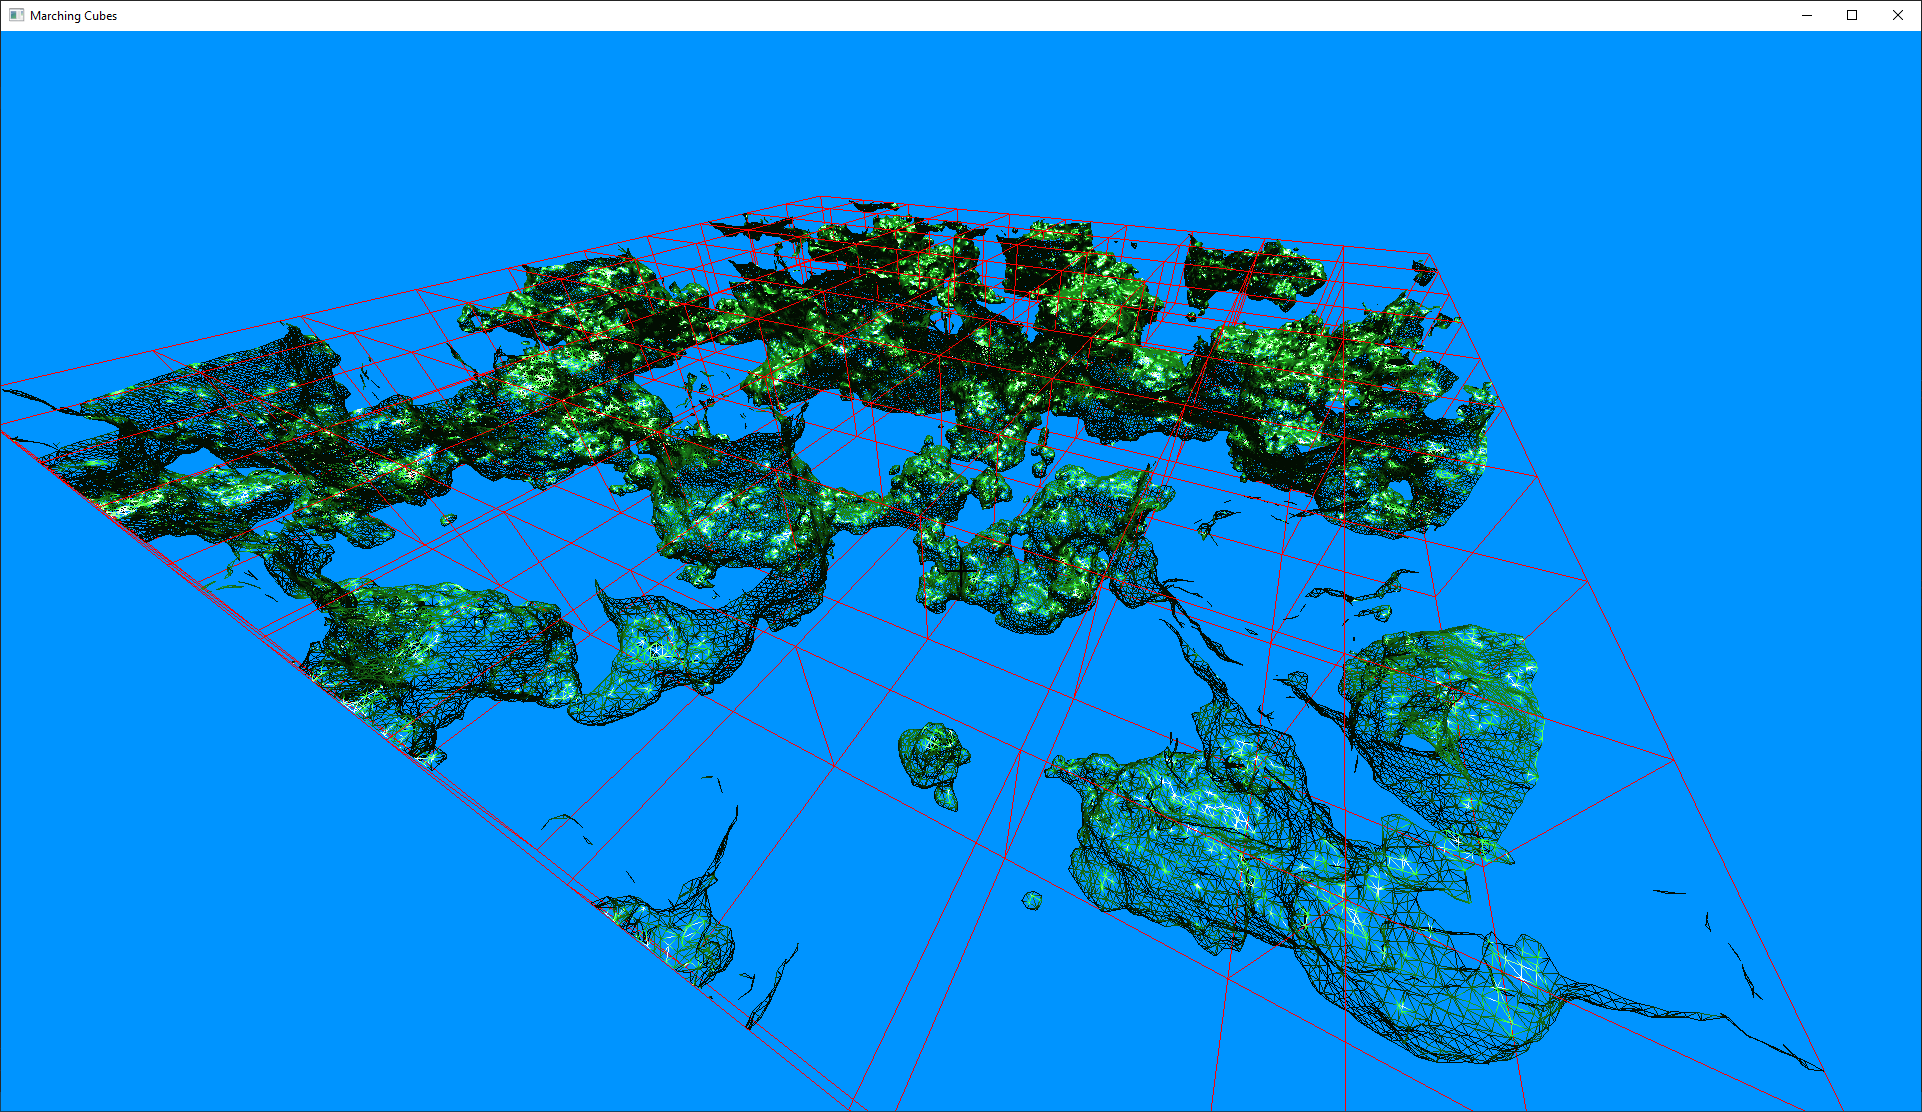
\includegraphics[width=\textwidth]{10x10_wireframe.png}
  \caption{An example of the 3D noise generated by these tests. This figure shows a wireframe of the 10x1x10 chunk test, with backface culling enabled.}
\end{figure}

\subsection{LOD system}
Even with a much more efficient GPU implementation of the Marching Cubes algorithm, when attempting to generate very large areas of geometry, it becomes infeasible to generate and render a uniform grid of Marching Cubes chunks. Furthermore, generating large amounts of triangles very far away from the camera is unnecessary, since the detail will not be visible. For this reason, it is necessary to have a dynamic level of detail (LOD) system.

\subsubsection{Octree}
To implement a versatile LOD system, an octree data structure is used. %TODO - explain an octree?
Each octree node represents a cuboid of space, such that the root node of the octree represents the entire renderable world, and the 8 children of an octree node equally divide the space represented by the parent node into octants. Each leaf node contains a reference to a chunk of generated geometry, as described in section \ref{section:mc_gpu}. The depth of the octree in any given region corresponds to the level of detail at which that region will have geometry generated. Each Marching Cubes chunk is generated with the same number of grid cells, regardless of the level of detail it is being generated for. However, the size of the grid cells doubles for each detail level increase. Using an octree provides versatility since any condition can be used to set the level of detail at a specific point in space. For example, it will be desirable to use the maximum level of detail near physics objects, so the physics collision is as accurate as possible, even if the camera is very far away.

\begin{figure}[H]
  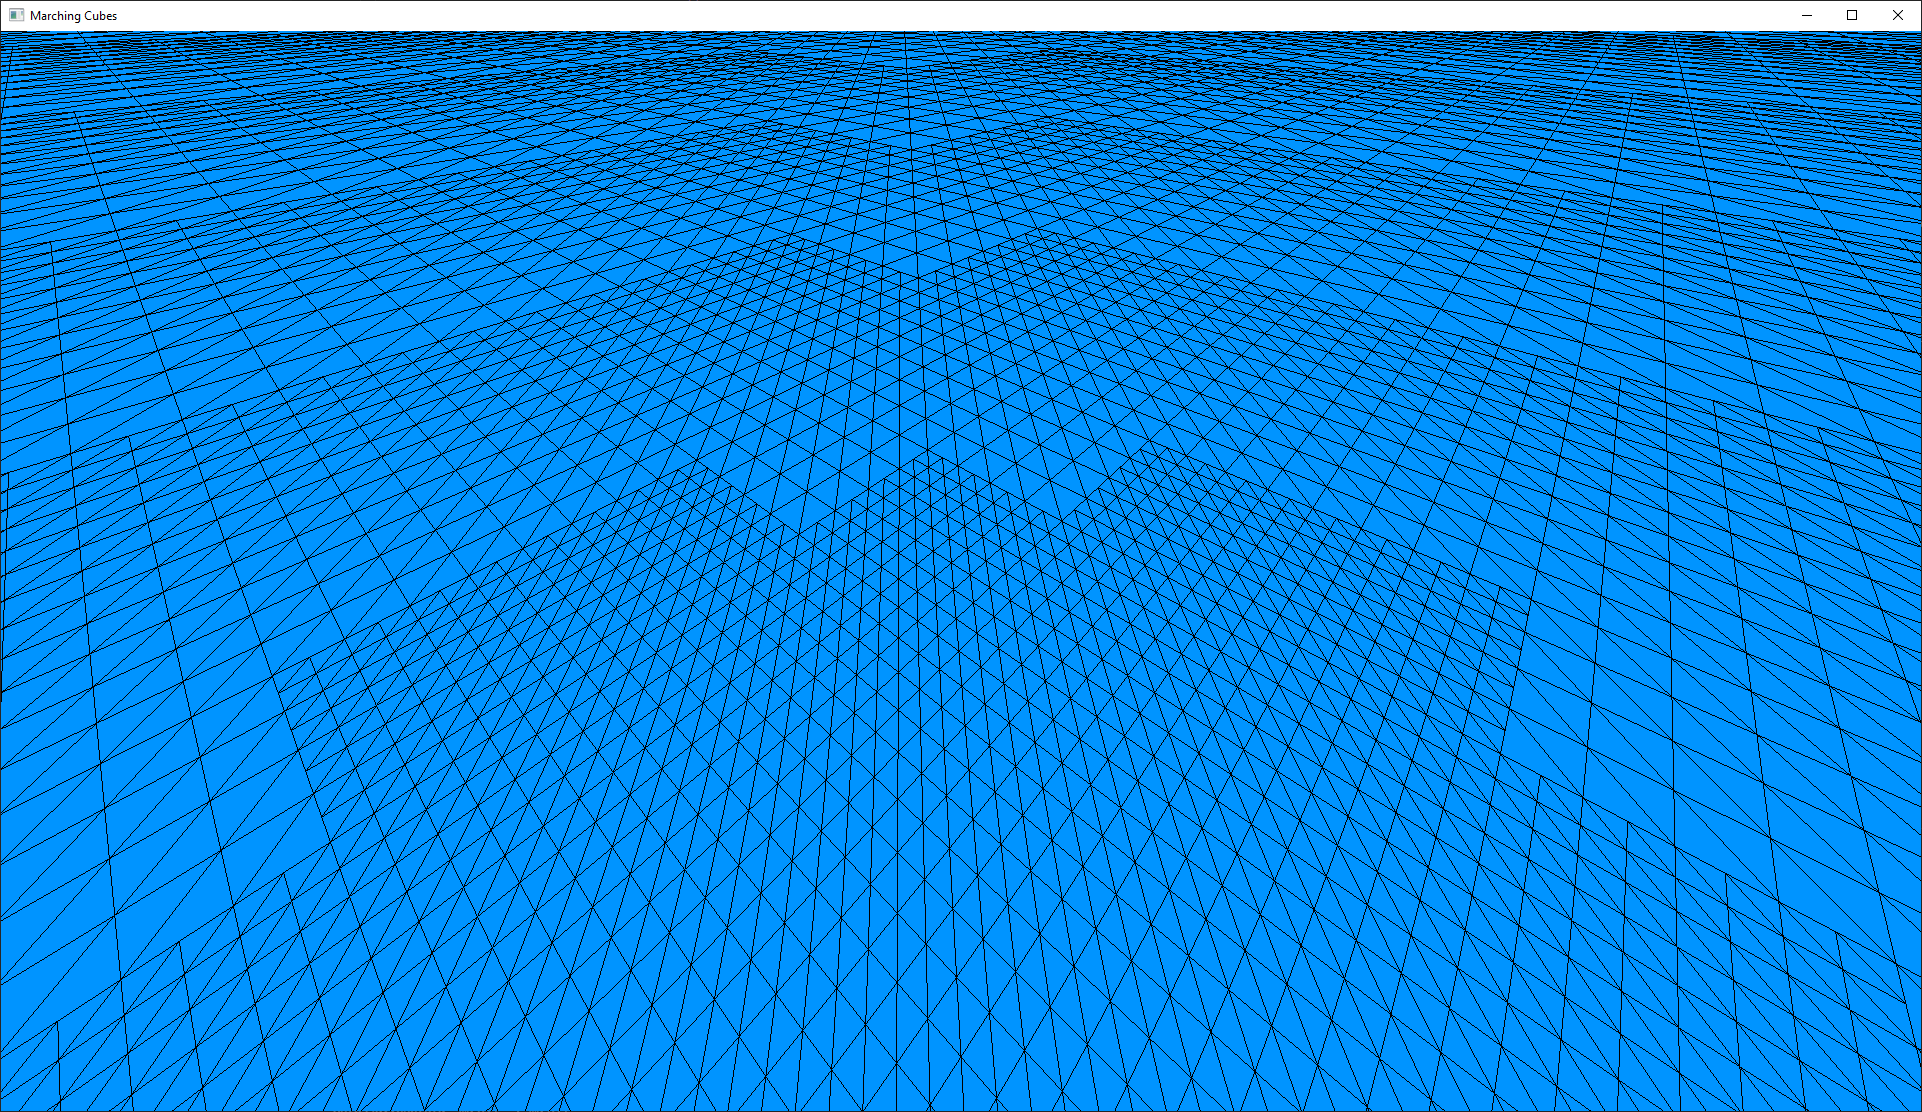
\includegraphics[width=\textwidth]{octree_plane.png}
  \caption{A plane SDF being generated using this octree LOD system. Here, the chunk size is $4^3$. The level of detail is configured to decrease as the distance from the camera increases.}
\end{figure}

When the octree changes, the level of detail at various points changes. The geometry currently generated at those points will be the wrong level of detail, and is considered invalid. The Marching Cubes chunks are deleted, and the region is completely regenerated at the correct level of detail.

\subsubsection{Issue with the Marching Cubes algorithm and LOD systems}
Using the Marching Cubes algorithm with multiple different grid cell sizes causes undesirable cracks in the surface of the generated geometry on the boundary between chunks of different levels of detail. A demonstration of what causes this is shown in figure \ref{fig:cracks_demo}, and an example within my code is shown in figure \ref{fig:cracks2}.

\begin{SCfigure}[][h]
  \caption{An illustration of the cracks between different levels of detail in the Marching Cubes algorithm. This figure shows the faces of 2 adjacent grid cells. The exact surface represented by the SDF is shown in purple, and the dotted lines show edges that may be produced by the Marching Cubes algorithm at the level of detail of these grid cells, and the level below. When these 2 cases occur next to each other, the space in between the 2 dotted lines forms a crack in the geometry.}
  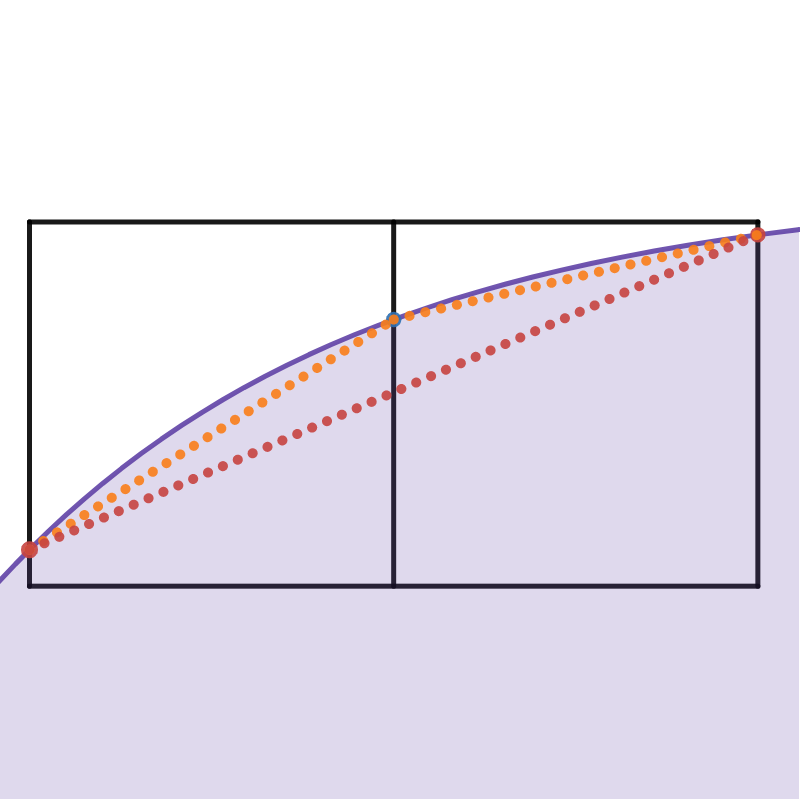
\includegraphics[width=0.5\textwidth]{cracks_demo.png}
  \label{fig:cracks_demo}
\end{SCfigure}

\begin{figure}[H]
  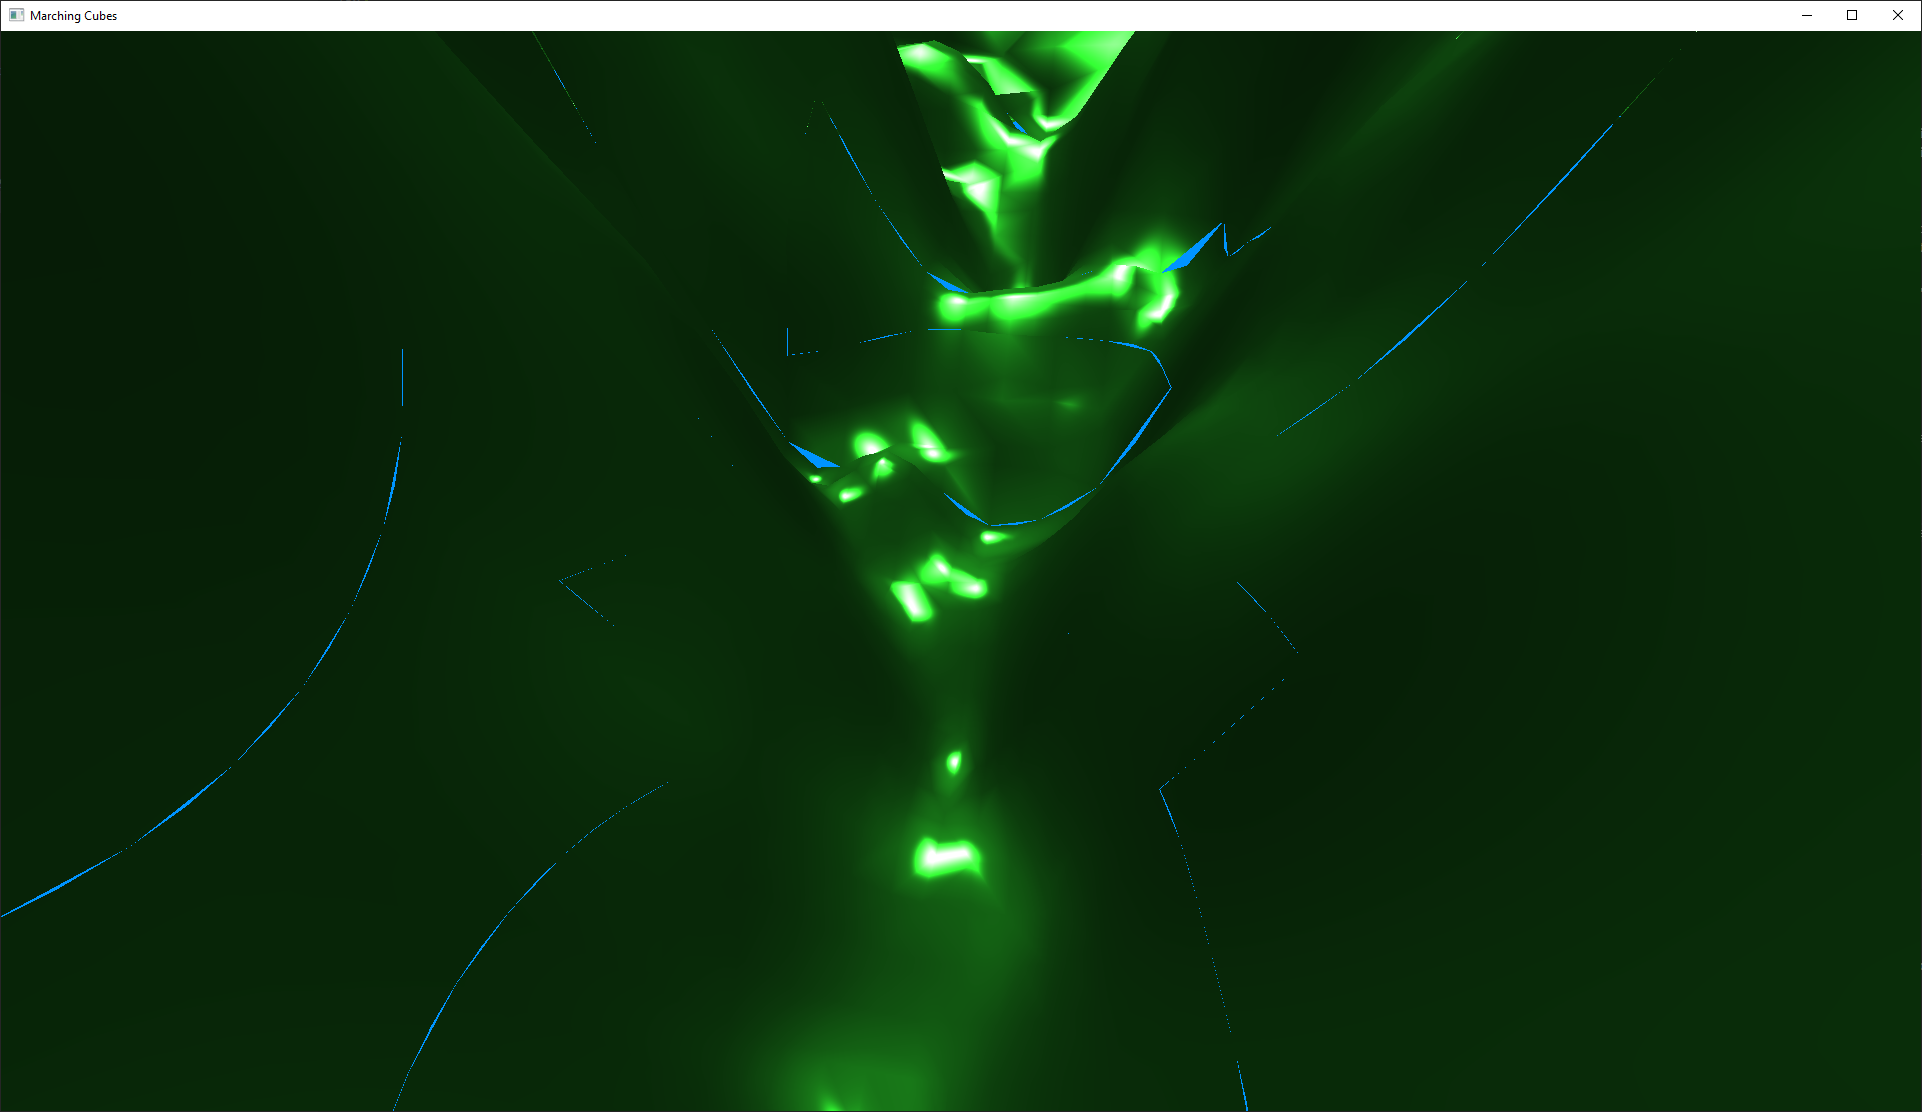
\includegraphics[width=\textwidth]{cracks2.png}
  \caption{An example with low chunk size, where the cracks in between levels of detail are clearly visible.}
  \label{fig:cracks2}
\end{figure}



\subsection{Transvoxel Algorithm}
%To go in this section - the edgeIndex part of the octree
\subsubsection{The problem it solves}
 - cracks in between chunks at different LOD
\subsubsection{How the algorithm works}
 - basically just a reference again\\
 - reference implementation is complicated so could do with explanation
\subsubsection{Adaption of the algorithm to GPU}
 - optimizations to make use of sequential generation have actually been removed\\
 - regardless, this is still pretty fast on the GPU\\
 - similar approach to parallel marching cubes\\
\subsubsection{More issues}
- zero width triangles\\
- edge cases where it still goes wrong (maybe a way to fix this by revisiting the octree)\\

\subsection{Terrain Modification}
\subsubsection{Strategy}
 - adding or removing primitives using SDF operations\\
 - regenerating chunks\\
 - when to regenerate chunks, and which ones\\
 - how many primitives is reasonable before slowdown due to SDF evaluation?\\
 - bounding boxes of primitives to increase this limit - dont need to evaluate parts not affected\\
 
 \subsection{Physics}
 - Just use bullet physics - well-known and optimized library\\
 - zero-width triangles havent turned out to be a problem so far\\
 - generating physics meshes is slow - need to find a solution to this\\
 - In fact, physics is currently the *slowest* part of this...\\
 \subsubsection{SDF-based physics}
 - perhaps look at this - might be a struggle because of non-exact SDFs, and how would we do it for anything that isn't a sphere anyway?
 
 \section{Implementation}
  - C++ with fairly low-level opengl libraries\\
  - key code probably in design section already\\
  - section for the ``boring bits'' of the implementation, rather than key ideas\\
  - perhaps section to explain other things that needed bugfixes?\\
  - something tying it all together?
  
\section{Conclusion}
 - demonstration of final product\\
 - conclusion\\
 - somehting about future work?

%\paragraph{paragraph}
%\subparagraph{subparagraph}

\bibliography{mc}
\end{document}